%----------------------------------------------------------------------------------------
%	PACKAGES AND DOCUMENT CONFIGURATIONS
%----------------------------------------------------------------------------------------

\documentclass{article}


\usepackage{graphicx} % Required for the inclusion of images
\usepackage{subfigure} % Required for the inclusion of images
\usepackage{natbib} % Required to change bibliography style to APA
\usepackage{amsmath} % Required for some math elements 
\usepackage{listings}
\usepackage{fontspec}
\usepackage{graphicx}
\usepackage[usenames]{xcolor}
\newfontfamily\monaco{Monaco}
\lstdefinelanguage{Y86}{
    morekeywords={irmovl, call, halt, xorl, jmp, ret, mrmovl, addl, jne, andl, pushl, rmmovl, subl, popl, je, iaddl, jl, jle, jg, jge, leave,
    esp, edi, eax, ebp, ecx, ebx, edx, esi,
    align, long, pos},
    sensitive=false,
    morecomment=[l]{#}
}
\lstset{ %
    language=Y86,                % the language of the code
    basicstyle=\small\monaco,           % the size of the fonts that are used for the code
    numbers=left,                   % where to put the line-numbers
    numberstyle=\tiny\color{gray},  % the style that is used for the line-numbers
    stepnumber=1,                   % the step between two line-numbers. If it's 1, each line 
                                    % will be numbered
    numbersep=5pt,                  % how far the line-numbers are from the code
    backgroundcolor=\color{white},      % choose the background color. You must add \usepackage{color}
    showspaces=false,               % show spaces adding particular underscores
    showstringspaces=false,         % underline spaces within strings
    showtabs=false,                 % show tabs within strings adding particular underscores
    frame=single,                   % adds a frame around the code
    rulecolor=\color{black},        % if not set, the frame-color may be changed on line-breaks within not-black text (e.g. commens (green here))
    tabsize=2,                      % sets default tabsize to 2 spaces
    captionpos=b,                   % sets the caption-position to bottom
    breaklines=true,                % sets automatic line breaking
    breakatwhitespace=false,        % sets if automatic breaks should only happen at whitespace
    title=\lstname,                 % show the filename of files included with \lstinputlisting;
                                    % also try caption instead of title
    keywordstyle=\color{blue},          % keyword style
    commentstyle=\color[RGB]{0,96,96},       % comment style
    stringstyle=\color{mauve},         % string literal style
    escapeinside={\%*}{*)},            % if you want to add LaTeX within your code
    morekeywords={*,...},              % if you want to add more keywords to the set
    }


%\usepackage{times} % Uncomment to use the Times New Roman font

%----------------------------------------------------------------------------------------
%	DOCUMENT INFORMATION
%----------------------------------------------------------------------------------------

\title{\textbf{Project 1: Optimizing the Performance of a Pipelined Processor}} % Title

\author{Yanjie Ze , Zhenyu Tang\\
 519021910706 , 519021910891\\
\\ \{zeyanjie, tang\_zhenyu\}  \textit{@sjtu.edu.cn} \\
   } % Author name and email

\date{\today} % Date for the report

\begin{document}

\maketitle % Insert the title, author and date

\section{Introduction}

\hspace{1 em}
\par In this project, the task consists of 3 parts:
\begin{enumerate}
    \item In Part A, we need to write Y86 assembly codes to implement 3 C functions. We wrote the code and checked the changed registers and memory.
    \item In Part B, we are required to implement \lstinline{iaddl} and \lstinline{leave} in the given pipelined processor. After that, we tested them on the ISA.
    \item In Part C, our goal is to optimize the performance of a pipelined processor. We combined Part B implementation here, and try 5 times improving the assembly code, using tricks like loop unrolling, preventing load use hazard, binary searching remaining loop number, rearranging jump instructions according to AT (Always Taken strategy), reaching final $CPE=8.93$.
\end{enumerate}

\textbf{Arrangment:} Yanjie Ze mainly took charge of finishing the coding part, and Zhenyu Tang mainly took charge of the report. To be more precise:
\begin{enumerate}
    \item Ze first solved Part A and Part B. Then Tang also finished separately in Part A and Part B, and checked whether the solution of Ze was correct.
    \item Ze finished Part C with $CPE=9.21$, using three tricks and one night. Then Tang followed Ze's solution and began the writing of the final report.
    \item Tang rewrote the binary search code in Part C based on Ze's solution and then added another trick getting $CPE=8.93$ , after which he finished the final report, together with Ze's participation.
\end{enumerate}
\par The final version of project code consists of Tang's Part A, Ze's Part B, and Ze's Part C with Tang's modification.
\section{Experiments}

\subsection{Part A}

\subsubsection{Analysis}
\hspace{1 em}
\par In this part, we are required to translate $3$ functions written in C into Y86 assembly language, namely \lstinline{sum_list()}, \lstinline{rsum_list()} and \lstinline{copy_block()}.
\par Implementing \lstinline{sum_list()} within \lstinline{sum.ys} is trivial referencing the codes on CS:APP book Fig. 4-7 with changing all the instructions to that of double words operands.
As for \lstinline{rsum_list()}, we implemented a recursive function using the stack. Therefore, we need to \lstinline{pushl} the temporal data and then after calling the function \lstinline{popl} them out and do the computation.
For \lstinline{copy_block()}, we copy data sized \lstinline{len} from \lstinline{src} to \lstinline{dest}.
\par In all of the above implementations, we cannot change the callee-saved registers. We need to push them into the stack before usage and afterwards pop and resume them.

\subsubsection{Code}

\begin{enumerate}
    \item Core part of \lstinline{sum.ys}
    \begin{lstlisting}
# ...
# int sum_list(list_ptr ls)
# ls in %edi
sum_list:
        pushl %ebp                  # Save the callee-saved register
        xorl %eax, %eax             # int val = 0;
        jmp test
loop:
        mrmovl (%edi), %ebp         # Get ls->val
        addl %ebp, %eax             # val += ls->val;
        mrmovl 4(%edi), %edi        # ls = ls->next;          
test:
        andl %edi, %edi             # Judge on ls
        jne loop                    # Stop when %edi is zero
        popl %ebp                   # Resume the callee-saved register
        ret
# ...
    \end{lstlisting}
    \item Core part of \lstinline{rsum.ys}
    \begin{lstlisting}
# ...
# int rsum_list(list_ptr ls)
# ls in %edi
rsum_list:
        xorl %eax, %eax             # int val = 0;
        xorl %ecx, %ecx             # Prevent problems
        andl %edi, %edi             # Judge on input
        je finish
        mrmovl (%edi), %eax         # int val = ls->val;
        pushl %eax                  # Save
        mrmovl 4(%edi), %edi        # ls = ls->next;
        call rsum_list
        popl %ecx
finish:
        addl %ecx, %eax
        ret
# ...
    \end{lstlisting}
    \item Core part of \lstinline{copy.ys}
\begin{lstlisting}
# ...
# int copy_block(int *src, int *dest, int len)
# src in %edi, dest in %esi, len in %edx
copy_block:
        pushl %ebp                  # Save callee-saved registers
        pushl %ebx
        irmovl $4, %ecx             # Save constant 4 since Y86 only supports addition and substraction on registers
        irmovl $1, %ebx             # Save constant 1
        xorl %eax, %eax             # int result = 0;
        jmp test
loop:
        mrmovl (%edi), %ebp         # int val = *src;
        addl %ecx, %edi             # src++;
        rmmovl %ebp, (%esi)         # *dest = val;
        addl %ecx, %esi             # dest++;
        xorl %ebp, %eax             # result ^= val;
        subl %ebx, %edx             # len--;
test:
        andl %edx, %edx             # Judge on len
        jne loop                    # Stop when len = 0
        popl %ebx                   # Resume callee-saved registers
        popl %ebp
        ret
# ...
    \end{lstlisting}
\end{enumerate}

\subsubsection{Evaluation}
\begin{enumerate}
    \item For \lstinline{sum_list()}, as can be seen in Fig.~\ref{fig:sum_res}, \lstinline{%eax} is changed to \lstinline{0xcba}, and no callee-saved registers are changed, which is correct. Note that stack pointers are all set \lstinline{0x200} in the programs.
    \begin{figure}[h]
        \centering
        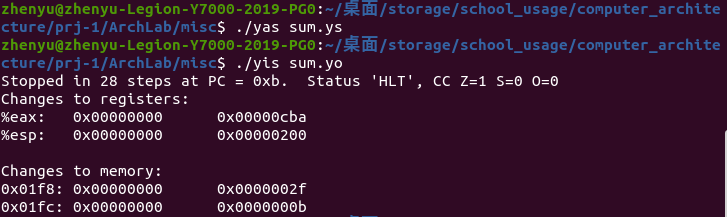
\includegraphics[width=0.9\textwidth]{sum_res.png}
        \caption{Result of sum.ys}
        \label{fig:sum_res}
    \end{figure}
    \item For \lstinline{rsum_list()}, as can be seen in Fig.~\ref{fig:rsum_res}, \lstinline{%eax} is also changed to \lstinline{0xcba}, and no callee-saved registers are changed, which is correct.
    \begin{figure}[h]
        \centering
        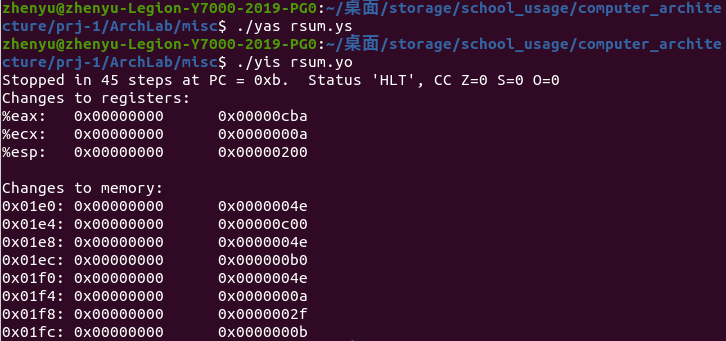
\includegraphics[width=0.9\textwidth]{rsum_res.png}
        \caption{Result of rsum.ys}
        \label{fig:rsum_res}
    \end{figure}
    \item For \lstinline{copy_block()}, as can be seen in Fig.~\ref{fig:copy_res}, the data are copy to the correct place and the return number is \lstinline{0xcba}.
    \begin{figure}[h]
        \centering
        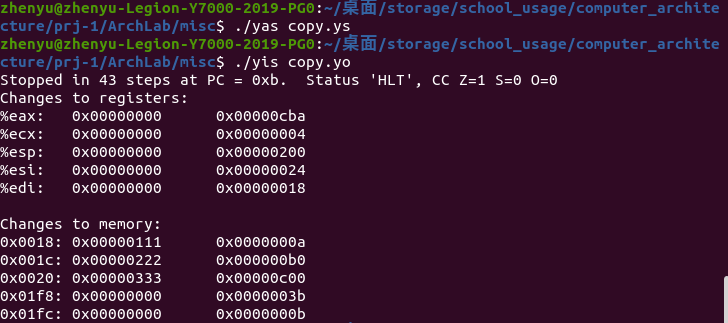
\includegraphics[width=0.9\textwidth]{copy_res.png}
        \caption{Result of copy.ys}
        \label{fig:copy_res}
    \end{figure}
\end{enumerate}

\subsection{Part B}

\subsubsection{Analysis}
\hspace{1 em

}
\par In this part, we are required to implement \lstinline{iaddl} instruction within the existing processor description in HCL. The instruction uses an immediate and a value of a register respectively as the ALU input, does addition and writes to a register. Therefore, we simply add \lstinline{IIADDL} into the corresponding code parts. 
\subsubsection{Code}

\begin{lstlisting}[language=python]
# ...
bool instr_valid = icode in 
	{ INOP, IHALT, IRRMOVL, IIRMOVL, IRMMOVL, IMRMOVL,
	       IOPL, IJXX, ICALL, IRET, IPUSHL, IPOPL, IIADDL };

# Does fetched instruction require a regid byte?
bool need_regids =
	icode in { IRRMOVL, IOPL, IPUSHL, IPOPL, 
		     IIRMOVL, IRMMOVL, IMRMOVL, IIADDL };

# Does fetched instruction require a constant word?
bool need_valC =
	icode in { IIRMOVL, IRMMOVL, IMRMOVL, IJXX, ICALL, IIADDL};
# ...
## What register should be used as the B source?
int srcB = [
	icode in { IOPL, IRMMOVL, IMRMOVL, IIADDL } : rB;
	# ...
];

## What register should be used as the E destination?
int dstE = [
	icode in { IRRMOVL } && Cnd : rB;
	icode in { IIRMOVL, IOPL, IIADDL} : rB;
	# ...
];
# ...
## Select input A to ALU
int aluA = [
	icode in { IRRMOVL, IOPL } : valA;
	icode in { IIRMOVL, IRMMOVL, IMRMOVL,IIADDL } : valC;
	# ...
];

## Select input B to ALU
int aluB = [
	icode in { IRMMOVL, IMRMOVL, IOPL, ICALL, 
		      IPUSHL, IRET, IPOPL,IIADDL } : valB;
	# ...
];
# ...
## Should the condition codes be updated?
bool set_cc = icode in { IOPL, IIADDL };
# ...
\end{lstlisting}

\subsubsection{Evaluation}
\hspace{1 em}
\par As can be seen in Fig.~\ref{fig:partb_test}, all the 870 ISA Checks, including \lstinline{iaddl} and \lstinline{leave}, succeed.
\begin{figure}[h]
    \centering
    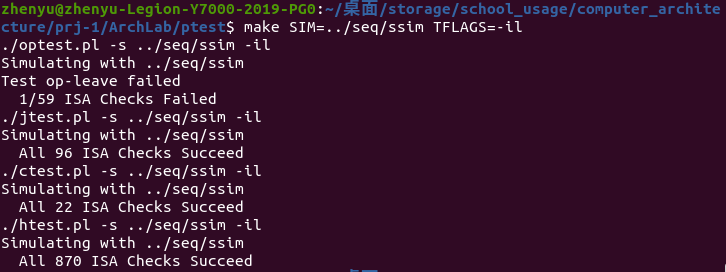
\includegraphics[width=0.9\textwidth]{partb_test.png}
    \caption{Test on Part B}
    \label{fig:partb_test}
\end{figure}

\subsection{Part C}

\subsubsection{Analysis}
\hspace{1 em}
\par In this part, we are required to optimize the performance of a pipelined processor on a function. We can optimize it on both the processor and the assembly code. The improvement history can be seen in Fig.~\ref{fig:cpe_down_hist}.
\begin{figure}[h]
    \centering
    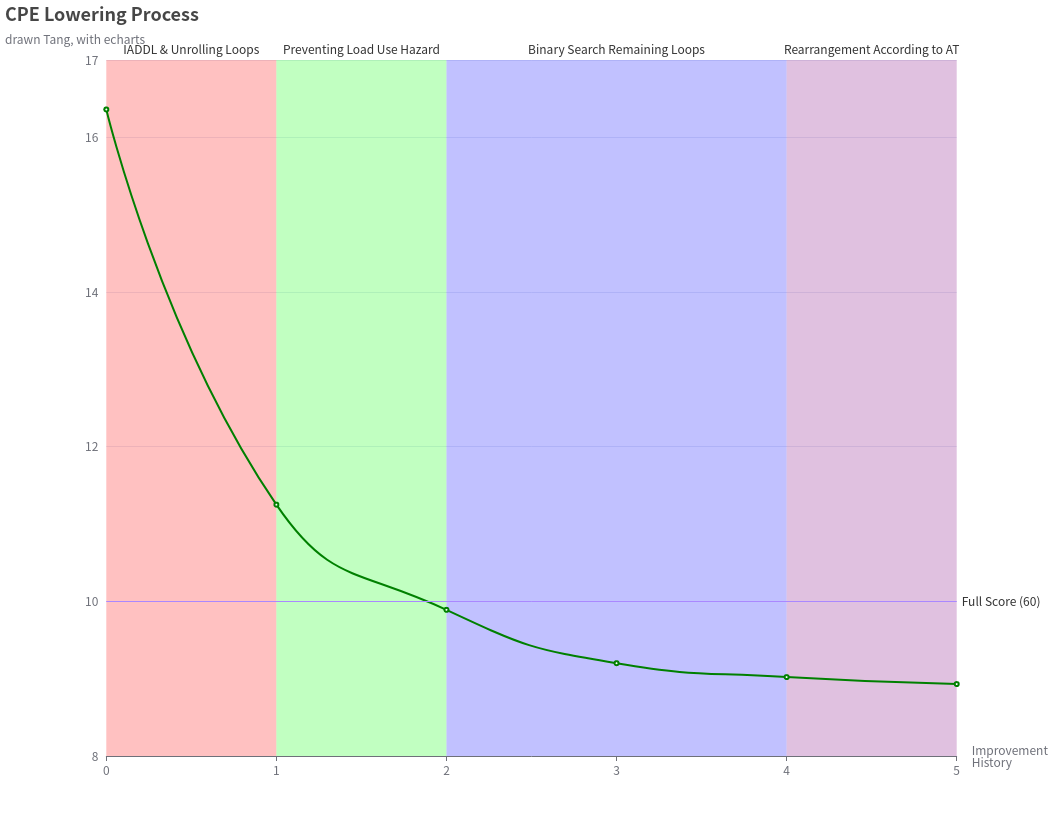
\includegraphics[width=1.0\textwidth]{CPE Lowering Process.png}
    \caption{The history of $CPE$ down}
    \label{fig:cpe_down_hist}
\end{figure}
\par On the processor part, we added the newly \textbf{implemented \lstinline{iaddl}} to the pipeline, with which we were able to directly add immediates to registers rather than loading them into the registers first. Since in the assembly part, we would try our best to avoid load-use hazard, optimization on load-use hazard in this part sees no much improvement in test, which we discarded.
\par On the assembly code, we first did \textbf{loop unrolling} and checked the best version of unrolling. As can be seen in Tab.~\ref{tab:unroll_res}, unrolling to \textbf{6 times} outperforms the other, and therefore we chose it.
\begin{table}[h]
    \centering
    \begin{tabular}{c|cccccccc}
         Unroll times & 1 & 4 & 5 & 6 & 7 & 8 & 10 & 12 \\
         \hline
        Score (/60)& 0 & 27.2 & 29.5 & 30.0 & 29.4 & 28.2 & 25.5 & 21.9 \\
        $CPE$ & 16.36 & 11.37 & 11.27 & 11.25 & 11.27 & $>$11.37 & $>$11.37 & $>$11.37
    \end{tabular}
    \caption{Performance of unrolling}
    \label{tab:unroll_res}
\end{table}
\par And then, we \textbf{prevented the load use hazard} by using two registers to store the data and loading aforehand. In the loop we load data in one register and switch to another to do operation on the previously loaded data, thus preventing bubbles and lowering $CPE$. In this case, the best unrolling time is supposed to be $4\sim 6$ in Tab.~\ref{tab:hazard_res}.
\begin{table}[h]
    \centering
    \begin{tabular}{c|ccccc}
         Unroll times & 3 & 4 & 5 & 6 & 7 \\
         \hline
         Improved score ($/60$)& 59.8 & 60 & 60 & 60 & 59.4\\
         Improved $CPE$& 10.01 & 9.89 & 9.90 & 9.95 & 10.03
    \end{tabular}
    \caption{Performance after preventing the load use hazard}
    \label{tab:hazard_res}
\end{table}
\par For the rest part of the loop besides unrolling, we did a \textbf{binary search} and get the remaining number of loops and then unroll them again. Here we get $CPE=9.21$ for unrolling 6 times, and $CPE=9.20$ for unrolling 8 times. Further rewriting the binary searching process we made it down to $CPE=9.02$.
\par Another trick is to \textbf{arrange the conditional jump instructions}. As can be seen from the assignment of \lstinline{bubble}s in the pipeline, the strategy used to predict a branch is \textbf{AT (Always Taken)} rather than the predict not taken strategy we used in implementing the MIPS pipelined processor. Hence in the binary search tree we arrange \lstinline{je} after \lstinline{jl} etc. since the latter contains more cases and is more probable to be taken. This trick helped lower $CPE$ from $9.02$ to less than $8.93$.
\par The critical part here is \textbf{trade-offs}. Unrolling more cycles will increase the performance, but also enlarge the instructions size. Moreover, unrolling more cycles will also increase the overhead of binary searching since the remain cases go up in numbers. Also, the arrangement according to AT is also a trade-off where we supposed the data to be uniformly distributed and hence chose the seemingly better 

\subsubsection{Code}

The following is the main part of implementation codes.

\begin{lstlisting}[language=Y86]
# ...
# Loop header
xorl %eax,%eax # count = 0;
iaddl $-6, %edx # len = len - 6
jl restjudge # if len<0, goto rest:

loop1: mrmovl (%ebx), %esi # val1
mrmovl 4(%ebx), %edi # val2
rmmovl %esi, (%ecx) # store val1
andl %esi, %esi # val1 <=0?
jle loop2 # if so, go to next loop
iaddl $1, %eax # count ++

loop2: mrmovl 8(%ebx), %esi # val1
rmmovl %edi, 4(%ecx) # store val2
andl %edi, %edi # val2 <=0?
jle loop3 # if so, go to next loop
iaddl $1, %eax # count ++

# The rest loops are similar to the above two, here omitted
# ...

loop6: 
rmmovl %edi, 20(%ecx) # store val2
andl %edi, %edi # val2 <=0?
jle update # if so, go to update, since this is the final loop
iaddl $1, %eax # count ++

update: iaddl $24, %ebx # update
iaddl $24, %ecx # update
iaddl $-6, %edx # len -= 6
jge loop1 # if len >= 0, go to new loop1

### rest loop ###
# binary search
# rearranged jl, jg and je according to AT
restjudge:
	iaddl $3, %edx
	jl searchleft
	jg searchright
	jmp restloop3
searchright:
	iaddl $-1, %edx
	je restloop4
	jmp restloop5
searchleft:
	iaddl $2, %edx
	je restloop1
	jg restloop2
	jmp Done
### search finish ###

### begin unrolling ###
restloop1: mrmovl (%ebx), %esi 
rmmovl %esi, (%ecx)
andl %esi, %esi
jle Done # finish
iaddl $1, %eax 
jmp Done

restloop2: mrmovl (%ebx), %esi # val1
mrmovl 4(%ebx), %edi # val2
rmmovl %esi, (%ecx) # store val1
andl %esi, %esi # val1 <=0?
jle restloop21 # if so, go to next loop
iaddl $1, %eax # count ++

restloop21: rmmovl %edi, 4(%ecx)
andl %edi, %edi
jle Done
iaddl $1, %eax
jmp Done

# the other rest loops are alike, here omitted

# ...
\end{lstlisting}

\subsubsection{Evaluation}
\begin{enumerate}
    \item We check the correctness like below:
\begin{lstlisting}[language=bash]
zhenyu@zhenyu-Legion-Y7000-2019-PG0:/storage/school_usage/computer_architecture/prj-1/ArchLab/pipe$ ./correctness.pl -p
Simulating with pipeline simulator psim
	ncopy
0	OK
# omit the other output OKs
64	OK
128	OK
192	OK
256	OK
68/68 pass correctness test
\end{lstlisting}
    \item And then check the copied length:
\begin{lstlisting}
zhenyu@zhenyu-Legion-Y7000-2019-PG0:/storage/school_usage/computer_architecture/prj-1/ArchLab/pipe$ ./check-len.pl < ncopy.yo
ncopy length = 678 bytes
\end{lstlisting}
    \item And then the CPE, the final CPE is around $8.93$:
\begin{lstlisting}
zhenyu@zhenyu-Legion-Y7000-2019-PG0:/storage/school_usage/computer_architecture/prj-1/ArchLab/pipe$ ./benchmark.pl
	ncopy
0	40
1	39	39.00
2	48	24.00
3	53	17.67
# omit the outputs
60	414	6.90
61	413	6.77
62	422	6.81
63	427	6.78
64	434	6.78
Average CPE	8.92
Score	60.0/60.0
\end{lstlisting}
\end{enumerate}

\section{Conclusion}

\subsection{Problems}

During the project, we met several obstacles and overcame them:
\begin{enumerate}
    \item When referencing the codes on CS:APP writing Part A, Tang found that the YAS assembler triggered an error \lstinline{Invalid line}. Double checking the codes on book and the provided test data, he figured out that the data size mismatch that of the operators in the book. Hence, he changed all the operators suffixed ``q'' to ``l'' and the problem was solved.
    \item When trying Part C at first, Tang encountered a problem that using \lstinline{iaddl} the $CPE$ directly goes down to about $2$, which was seemingly impossible with just a few modifications. Checking the copied length he found that the \lstinline{iaddl} had not been implemented in the processor in Part C. Combining Part B solution in the pipelined processor in Part C he finally got the answer back to normal.
    \item When trying modifying on Ze's Part C solution, Tang tried optimizing the stalling and bubbles conditions. However, the trial saw barely any improvement, and afterwards he recognized that the load use hazard has already been prevented by Ze. Therefore, such trial is not expected to optimize a lot.
\end{enumerate}

\subsection{Achievements}

\hspace{1 em}

\par For Part A, our program works as expected on the tested data.
\par For Part B, our processor passed the test of all given 870 ISA checks.
\par For Part C, our project passed the correctness check, and yields a $CPE$ of $8.93$ or lower, almost half of that of the raw one. In the recent $10$ tests, $8.93$ occurs twice, $8.92$ occurs $7$ times, and $8.91$ occurs once.
\par In the project, we have our codes commented as fully as possible, making it more convenient to cooperate. Moreover, we worked with each other over GitHub for coding and Overleaf (SJTU) for report writing, getting more familiar using those tools.
\par We managed to bridge between what we have learned in the class and practice. With this project, we learned to write assembly codes, and writing a new hardware description language - HCL. More importantly, reading the pre-written HCL codes we learned about the implementation of pipelining in a CISC ISA, which is similar to our implementation on that of MIPS ISA, but with some noticeable differences like \lstinline{valP} to predict PC for the next instruction. We also gain a deeper view inside data hazard, strategies for solving control hazards and the compiler technique of loop unrolling
etc modifying on the assembly codes.

%----------------------------------------------------------------------------------------


\end{document}